\documentclass{standalone}
\usepackage{tikz}
\usetikzlibrary{positioning}

\begin{document}
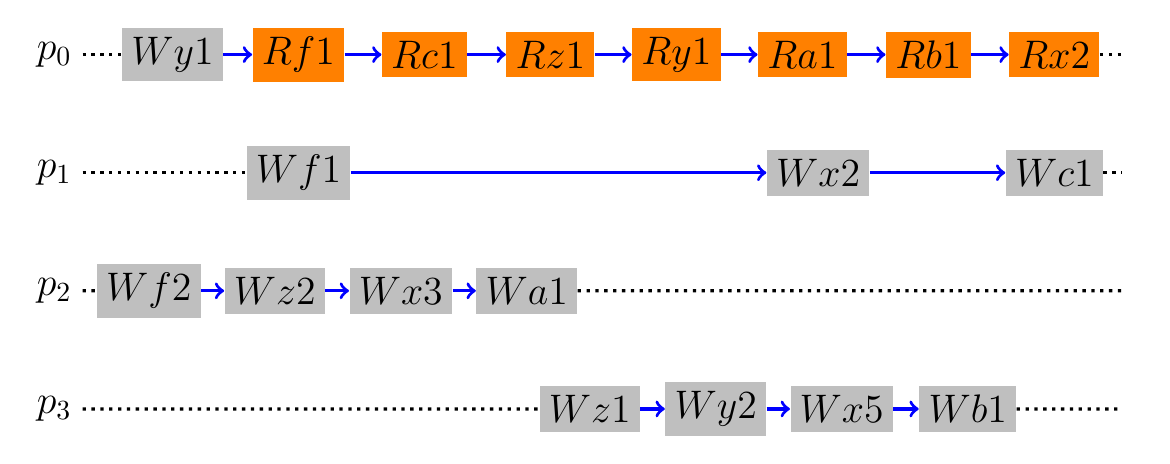
\begin{tikzpicture}[read/.style = {fill = orange, font = \Large}, 
write/.style = {fill = lightgray, font = \Large},
on grid, every node/.style = {node distance = 1.0cm and 1.6cm}, 
po/.style = {->, very thick, blue}]
%   	      \draw[step = {(1.5,1)}, style=help lines] (-1.5,0) grid (10.5,4);
	% process 0
	\begin{scope}[yshift = 4.0cm]
		\node (wy1) [write] at (0,0) {$Wy1$};
		\node (rf1) [read, right = of wy1] {$Rf1$};
		\node (rc1) [read, right = of rf1] {$Rc1$};
		\node (rz1) [read, right = of rc1] {$Rz1$};
		\node (ry1) [read, right = of rz1] {$Ry1$};
		\node (ra1) [read, right = of ry1] {$Ra1$};
		\node (rb1) [read, right = of ra1] {$Rb1$};
		\node (rx2) [read, right = of rb1] {$Rx2$};
	\end{scope}

	% process 1
	\begin{scope}
		\node (wf1) [write, node distance = 1.5cm, below = of rf1] {$Wf1$};
		\node (wx2) [write, node distance = 1.5cm and 3.0cm, below left = of rx2] {$Wx2$};
		\node (wc1) [write, node distance = 3.0cm, right = of wx2] {$Wc1$};
	\end{scope}

	% process 2
	\begin{scope}[]
		\node (wa1) [write, node distance = 3.0cm and 3.5cm, below left = of ra1] {$Wa1$};
		\node (wx3) [write, left = of wa1] {$Wx3$};
		\node (wz2) [write, left = of wx3] {$Wz2$};
		\node (wf2) [write, left = of wz2] {$Wf2$};
	\end{scope}

	% process 3
	\begin{scope}[]
		\node (wb1) [write, node distance = 4.5cm and 0.5cm, below right = of rb1] {$Wb1$};
		\node (wx5) [write, left = of wb1] {$Wx5$};
		\node (wy2) [write, left = of wx5] {$Wy2$};
		\node (wz1) [write, left = of wy2] {$Wz1$};
	\end{scope}

\begin{scope}[dotted, very thick, every node/.style = {font = \Large}]
  \node (lvnode) [node distance = 1.5cm, left = of wy1] {};
  \node (rvnode) [node distance = 1.0cm, right = of rx2] {};
  
  \node (p0) at (lvnode) {$p_0$};
  \draw (p0) -- (wy1);
  \node (rp0) at (rvnode) {};
  \draw (rx2) -- (rp0);

  \node (p1) [node distance = 1.5cm, below = of p0] {$p_1$};
  \draw (p1) -- (wf1);
  \node (rp1) [node distance = 1.5cm, below = of rp0] {};
  \draw (wc1) -- (rp1);

  \node (p2) [node distance = 1.5cm, below = of p1] {$p_2$};
  \draw (p2) -- (wf2);
  \node (rp2) [node distance = 1.5cm, below = of rp1] {};
  \draw (wa1) -- (rp2);

  \node (p3) [node distance = 1.5cm, below = of p2] {$p_3$};
  \draw (p3) -- (wz1);
  \node (rp3) [node distance = 1.5cm, below = of rp2] {};
  \draw (wb1) -- (rp3);
\end{scope}

% program order
\begin{scope}[]
  \draw[po] (wy1) -- (rf1);
  \draw[po] (rf1) -- (rc1);	  
  \draw[po] (rc1) -- (rz1);
  \draw[po] (rz1) -- (ry1);
  \draw[po] (ry1) -- (ra1);
  \draw[po] (ra1) -- (rb1);
  \draw[po] (rb1) -- (rx2);

  \draw[po] (wf1) -- (wx2);
  \draw[po] (wx2) -- (wc1);

  \draw[po] (wf2) -- (wz2);
  \draw[po] (wz2) -- (wx3);
  \draw[po] (wx3) -- (wa1);

  \draw[po] (wz1) -- (wy2);
  \draw[po] (wy2) -- (wx5);
  \draw[po] (wx5) -- (wb1);
\end{scope}

\end{tikzpicture}
\end{document}